\graphicspath{{../03Mathematics/pics/}}

\chapter{Mathematics}\label{ch:Mathematics}

\lettrine[lines=2]{\color{darkocre}I}{n} the previous chapter we
learned about numbers and various relations between them. As a
particular class of relations we discussed functions. We introduced
\emph{binary} and \emph{unary} functions and different ways
functions can be combined (\emph{composed}) to produce new
functions. We also learned
that functions can be
represented in various ways and that none of those different
representations defines
the concept of function completely. Each representation of a function
highlighted some important aspect of it.

\section{Arrows}

To arrive at the idea of vectors we will start with simple geometrical
objects -- arrows in a plane, as illustrated in the Figure \ref{fig:arrowsSpace}.

\begin{SCfigure}%[htbp]
  %\centering
  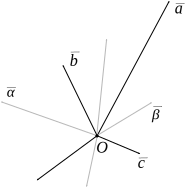
\includegraphics[scale=1.0]{arrowsSpace}
  \caption{Set of arrows starting at the same origin point $O$. All
    imaginable arrows taken as one set form the arrow space
    $\overset{\Rightarrow}{A}$.}
  \label{fig:arrowsSpace}
\end{SCfigure}

Symbolically, we will denote vectors by placing an arrow over letters:
\[
\vec{a}\,,\vec{b}\,,\vec{c}\,,\ldots\,,\vec{\alpha}\,,\vec{\beta}\,.
\]

\subsection{Dirac Notation}

\section{Scalar Product}

To arrive at the idea of vectors we will start with simple geometrical
objects -- arrows in a plane, as illustrated in the Figure \ref{fig:arrowsSpace}.

\section{Operators}

To arrive at the idea of vectors we will start with simple geometrical
objects -- arrows in a plane.
\[
\braket{\phi}{\phi}
\]
and
\[
\ketbra{\phi}{\phi}\,.
\]

\section{Spaces}

To arrive at the idea of vectors we will start with simple geometrical
objects -- arrows in a plane.
\[
\braket{\phi}{\phi}
\]
and
\[
\ketbra{\phi}{\phi}\,.
\]

\section*{Chapter Highlights}
{\setstretch{1.5}\chhc
  \it
\begin{itemize}
\item Arrows in a plane provide a simple model for vectors.
\item Arrows can be manipulated in ways analogous to numbers: Two arrows
  be added, an arrow can be ``scaled'' (stretched or compressed). Arrows form
  an algebra.
\item Basis is an extremely important concept. Basis is a set of
  objects (arrows) that can be used to ``build'' all other similar
  objects (arrows). At the same time, basis can not be used to build
  itself -- basis arrows are independent.
\end{itemize}
}
